\section*{سوال ۱}

شبیه سازی یک مثال
\lr{(Real-Time Scheduling)}
در
\lr{True Time}
در نرم افزار متلب و ارایه یک گزارش (رجوع به اسلاید شماره دو)

\section*{جواب سوال ۱}

\begin{comment}
\begin{figure}[h]
	\centering
	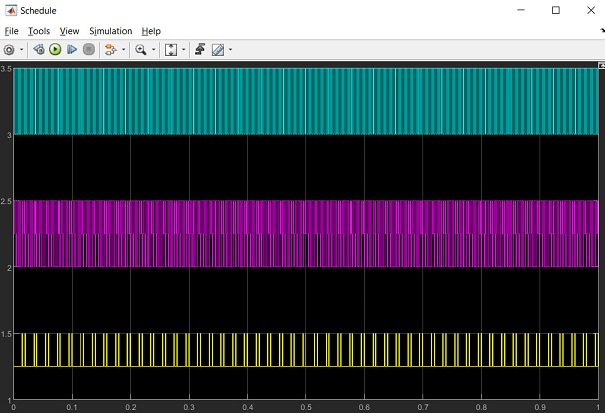
\includegraphics{6.jpg}
	\label{fig:label4}
\end{figure}
\end{comment}

\section*{گزارش کار با نرم‌افزار MATLAB و اجرای TrueTime}

در ابتدا، به دایرکتوری مورد نظر برای فعال‌سازی TrueTime در متلب مراجعه کردیم با این دستور:
\begin{figure}[h]
	\centering
	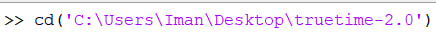
\includegraphics{12.jpg}
	\label{fig:label4}
\end{figure}


سپس، ماژول TrueTime با استفاده از دستور زیر فعال شده است:

\begin{figure}[h]
	\centering
	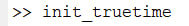
\includegraphics{13.jpg}
	\label{fig:label4}
\end{figure}

برای مشاهده محتوای دایرکتوری فعلی، از دستور \texttt{ls} استفاده شده است:

\begin{figure}[h]
	\centering
	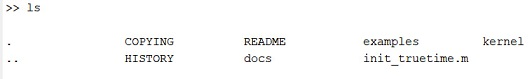
\includegraphics{14.jpg}
	\label{fig:label4}
\end{figure}

بعد از آن، به دایرکتوری \texttt{examples} و سپس به زیر دایرکتوری \texttt{threeservos} مراجعه شده است. در این قسمت، با کلیک روی فایل با فرمت slx ، شبیه‌سازی \texttt{threeservos} اجرا شده است.

\begin{figure}[H]
	\centering
	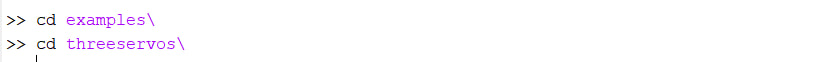
\includegraphics{15.jpg}
	\label{fig:label4}
\end{figure}

\newpage

\section*{بررسی فایل‌های داخل فولدر \lr{threeservos}}

با توجه به فایل‌های موجود در فولدر و فرمت‌ها و نام‌های موجود، فایل \texttt{threeservos.slx} فایل اصلی برنامه است. فایل‌های با پسوند \texttt{.slx} فایل‌های مدل‌سازی Simulink در MATLAB هستند و معمولاً برای شبیه‌سازی سیستم‌های کنترلی و دینامیکی استفاده می‌شوند.

فایل‌های دیگر با پسوند \texttt{.m} همگی اسکریپت‌ها یا توابع MATLAB هستند که توسط فایل \texttt{threeservos.slx} فراخوانی می‌شوند یا به تنهایی اجرا می‌شوند.

\begin{figure}[H]
	\centering
	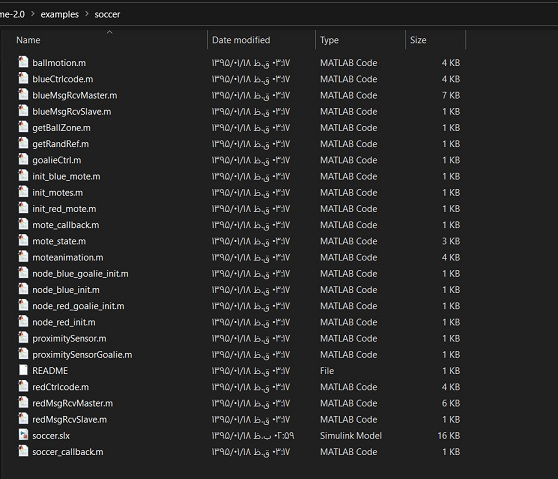
\includegraphics{2.jpg}
	\label{fig:label4}
\end{figure}

\newpage

\section*{محتویات فایل \lr{threeservos.slx}}

برای تشخیص دقیق‌تر، فایل \texttt{threeservos.slx} را در MATLAB باز کردیم و به محتوای آن نگاهی می‌اندازیم.

\begin{figure}[H]
	\centering
	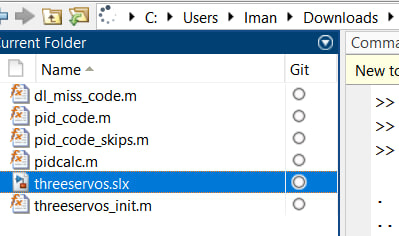
\includegraphics{4.jpg}
	\label{fig:label4}
\end{figure}

\begin{figure}[H]
	\centering
	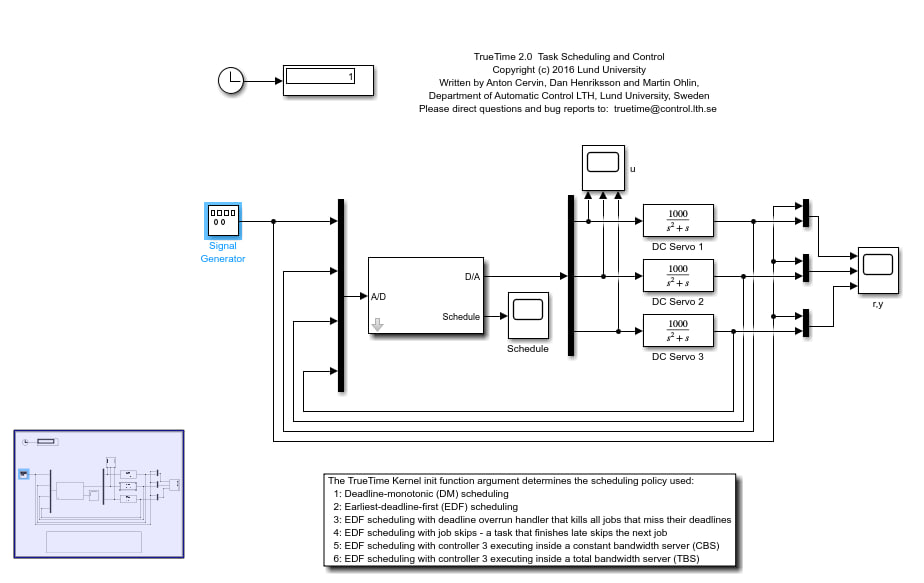
\includegraphics{17.jpg}
	\label{fig:label4}
\end{figure}

\newpage

\section*{تصاویر ران برنامه}

\begin{figure}[H]
	\centering
	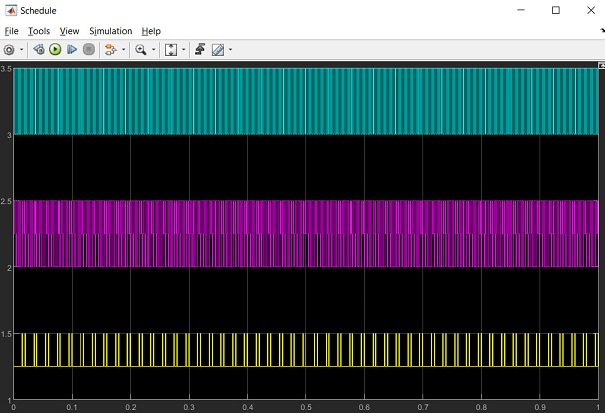
\includegraphics{6.jpg}
	\label{fig:label4}
\end{figure}

\begin{figure}[H]
	\centering
	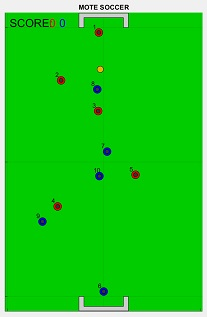
\includegraphics{7.jpg}
	\label{fig:label4}
\end{figure}

\begin{figure}[H]
	\centering
	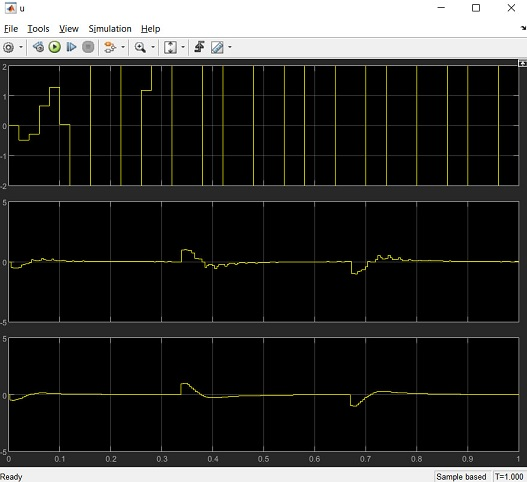
\includegraphics{8.jpg}
	\label{fig:label4}
\end{figure}

\begin{figure}[H]
	\centering
	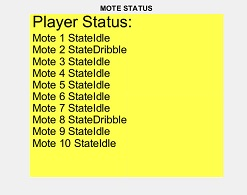
\includegraphics{9.jpg}
	\label{fig:label4}
\end{figure}

\begin{figure}[H]
	\centering
	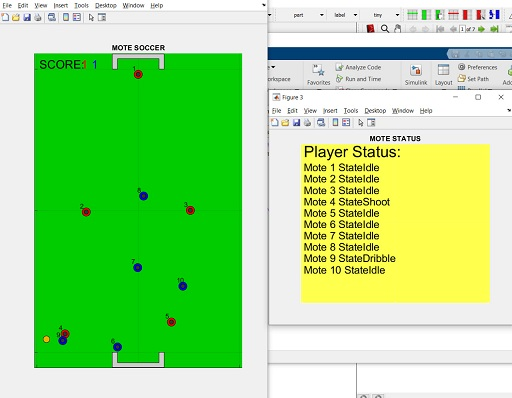
\includegraphics{10.jpg}
	\label{fig:label4}
\end{figure}

\newpage

\section*{کد \lr{threeservos_init.m}}

تابع فراخواننده‌ی این شبیه‌سازی در برنامه‌ی متلب:

\begin{figure}[H]
	\centering
	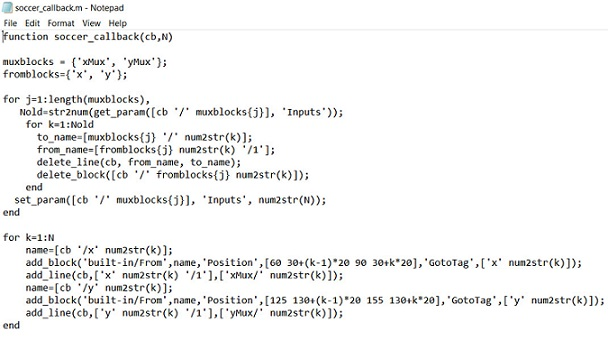
\includegraphics{16.jpg}
	\label{fig:label4}
\end{figure}

\newpage

\section*{روند ران کردن برنامه}

فولدر
\lr{truetime2}
را دریافت می‌کنیم و با اجرای دستورات مربوطه و وارد فولدر برنامه شدن و در نهایت کلیک روی فایل با فرمت slx ، برنامه ران می‌شود.

\section*{توضیح کد}

\item \textbf{اولیه‌سازی کرنل:} بسته به مقدار ورودی \texttt{arg}، کرنل TrueTime با سیاست زمان‌بندی متفاوتی اولیه‌سازی می‌شود. از جمله:
\begin{itemize}
	\item با \texttt{arg = 1}، سیاست زمان‌بندی DM (\textit{Deadline Monotonic}) استفاده می‌شود.
	\item با \texttt{arg = 2 , 3 , 5 , 6}، سیاست زمان‌بندی EDF (\textit{Earliest Deadline First}) به کار می‌رود.
	\item در حالت خاص \texttt{arg = 4}، یک رویه مدیریت تأخیر برای وظایف اجرایی در نظر گرفته می‌شود.
\end{itemize}

\item \textbf{تعریف پارامتر‌های وظیفه:} زمان شروع، دوره زمانی و نام‌های وظایف برای سه وظیفه کنترل PID تعیین می‌شوند.

\item \textbf{ایجاد وظایف:} برای هر یک از سه سیستم سروو، یک وظیفه پریودیک با پارامترهای مشخص شده ایجاد می‌شود. داده‌های هر وظیفه شامل پارامتر‌های کنترلی PID ، زمان دوره، و شناسه‌های کانال‌ها برای ورودی، خروجی و مقدار مورد نظر است.

\item \textbf{مدیریت وظایف با تأخیر:} بسته به مقدار \texttt{arg} ، اقدامات مختلفی برای مدیریت وظایف با تأخیر اتخاذ می‌شود، از جمله ایجاد دستگیره‌ها برای مدیریت تأخیرها و اختصاص وظایف به سیاست‌های زمان‌بندی مشخص.

\end{enumerate}

کد به پایان می‌رسد با اجرای این مراحل، که در آن سه وظیفه کنترل PID برای سروو‌ها ایجاد و مدیریت می‌شوند، و با توجه به سیاست زمان‌بندی انتخابی، عملکرد کلی کنترل تحت تأثیر قرار می‌گیرد.


\newpage

\section*{آموزش نصب و فعال‌سازی MATLAB ورژن \lr{2023a}}

\begin{enumerate}
	\item قبل از شروع نصب، اتصال به اینترنت را قطع می‌کنیم.
	\item فایل مورد نظر از حالت فشرده خارج شده است.
	\item فایل \lr{R2023a\_Windows.iso} را با استفاده از یک برنامه‌ی درایو مجازی Mount نموده و نصب را شروع می‌کنیم.
	\item فایل \texttt{Setup} را اجرا کرده و در قسمت \lr{Enter File Installation Key}، سریال گفته شده را وارد کردیم:
	
	\item در مرحله \lr{Select License File}، فایل \texttt{license.lic} واقع در پوشه‌ی \texttt{Crack} را انتخاب می‌کنیم.
	\item پس از نصب، نرم‌افزار را اجرا نمی‌کنیم.
	\item فایل \texttt{libmwlmgrimpl.dll} را از پوشه‌ی \texttt{Crack} به مسیر گفته شده کپی کردیم و فایل را در آن مسیر جایگزین می‌نماییم.
	کپی کرده و فایل موجود در آن مسیر را جایگزین می‌کنیم.
	\item حال می‌توانید نرم‌افزار را اجرا کنیم.
	\item در صورت نیاز به آپدیت، فایل آپدیت با فرمت \texttt{iso} را مانت کرده و فایل \texttt{Update.cmd} را اجرا می‌کنیم.
	\item مجدداً فایل \texttt{libmwlmgrimpl.dll} را جایگزین می‌کنیم.
\end{enumerate}
